\myheading{Quick introduction into modular arithmetic}

\leveldown{}

Modular arithmetic is an environment where all values are limited by some number (modulo).
Many textbooks has clock as example. Let's imagine old mechanical analog clock.
There hour hand points to one of number in bounds of 0..11 (zero is usually shown as 12).
What hour will be if to sum up 10 hours (no matter, AM or PM) and 4 hours?
10+4 is 14 or 2 by modulo 12.
Naively you can just sum up numbers and subtract modulo base (12) as long as it's possible.

Modern digital watch shows time in 24 hours format, so hour there is a variable in modulo base 24.
But minutes and seconds are in modulo 60 (let's forget about leap seconds for now).

Another example is US imperial system of measurement: human height is measured in feets and inches.
There are 12 inches in feet, so when you sum up some lengths, you increase feet variable each time you've got more than 12 inches.

Another example I would recall is password cracking utilities. Often, characters set is defined in such utilities.
And when you set all Latin characters plus numbers, you've got 26+10=36 characters in total.
If you brute-forcing a 6-characters password, you've got 6 variables, each is limited by 36.
And when you increase last variable, it happens in modular arithmetic rules: if you got 36, set last variable to 0 and increase penultimate
one. If it's also 36, do the same. If the very first variable is 36, then stop.
Modular arithmetic may be very helpful when you write multi-threading (or distributed) password cracking utility and you need to slice all passwords space by even
parts.

\myhrule{}

This is yet another application of modulo arithmetic, which many of us encountered in childhood.

Given a counting rhyme, like:

\begin{lstlisting}
    Eeny, meeny, miny, moe,
    Catch a tiger by the toe.
    If he hollers, let him go,
    Eeny, meeny, miny, moe.
\end{lstlisting}
( \url{https://en.wikipedia.org/wiki/Eeny,_meeny,_miny,_moe} )

... predict, who will be choosen.

If I'm correct, that rhyme has 16 items, and if a group of kids constist of, say, 5 kids, who will be choosen?
16 mod 5 = 1, meaning, the next kid after the one at whom counting had begun.

Or 7 kids, 16 mod 7 = 2. Count two kids after the first one.

If you can calculate this quickly, you can probably get an advantage by choosing a better place within a circle...

\myhrule{}

Now let's recall old mechanical counters which were widespread in pre-digital era:

\begin{figure}[H]
\centering
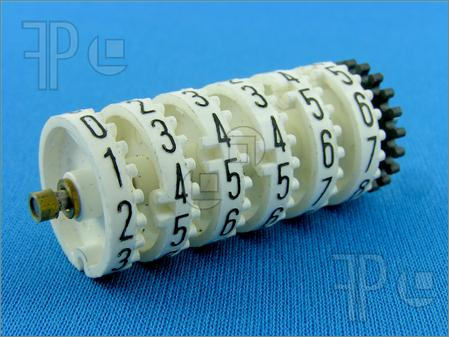
\includegraphics[scale=0.66]{modulo/counter.jpg}
\caption{The picture was stolen from \url{http://www.featurepics.com/} --- sorry for that!}
\end{figure}

This counter has 6 wheels, so it can count from 0 to $10^{6}-1$ or 999999.
When you have 999999 and you increase the counter, it will resetting to 000000---
this situation is usually understood by engineers and computer programmers as overflow.
And if you have 000000 and you decrease it, the counter will show you 999999.
This situation is often called ``wrap around''.
See also: \url{http://en.wikipedia.org/wiki/Integer_overflow}.

\myheading{Modular arithmetic on CPUs}

The reason I talk about mechanical counter is that CPU registers acting in the very same way, because this is, perhaps, simplest possible and efficient way
to compute using integer numbers.

This implies that almost all operations on integer values on your CPU is happens by modulo $2^{32}$ or $2^{64}$ depending on your CPU.
For example, you can sum up 0x87654321 and 0xDEADBABA, which resulting in 0x16612FDDB.
This value is too big for 32-bit register, so only 0x6612FDDB is stored, and leading 1 is dropped.
If you will multiply these two numbers, the actual result it 0x75C5B266EDA5BFFA, which is also too big, so only low 32-bit part is stored into destination
register: 0xEDA5BFFA. This is what happens when you multiply numbers in plain C/C++ language, but some readers may argue:
when sum is too big for register, CF (carry flag) is set, and it can be used after.
And there is x86 MUL instruction which in fact produces 64-bit result in 32-bit environment (in EDX:EAX registers pair).
That's true, but observing just 32-bit registers, this is exactly environment of modulo with base $2^{32}$.

Now that leads to a surprising consequence: almost every result of arithmetic operation stored in general purpose register of
32-bit CPU is in fact
remainder of division operation: result is always divided by $2^{32}$ and remainder is left in register.
For example, 0x16612FDDB is too large for storage, and it's divided by $2^{32}$ (or 0x100000000).
The result of division (quotient) is 1 (which is dropped) and remainder is 0x6612FDDB (which is stored as a result).
0x75C5B266EDA5BFFA divided by $2^{32}$ (0x100000000) produces 0x75C5B266 as a result of division (quotient) and 0xEDA5BFFA as a remainder, the latter is stored.

And if your code is 32-bit one in 64-bit environment, CPU registers are bigger, so the whole result can be stored there,
but high half is hidden behind the scenes -- because no 32-bit code can access it.

By the way, this is the reason why remainder calculation is often called "division by modulo".
C/C++ has a percent sign (``\%'') for this operation, but some other PLs like Pascal and Haskell has "mod" operator.

Usually, almost all sane computer programmers works with variables as they never wrapping around and value here is always in some limits which
are defined preliminarily.
However, this implicit division operation or "wrapping around" can be exploited usefully.

\myheading{Remainder of division by modulo $2^{n}$}

... can be easily computed with AND operation.
If you need a random number in range of 0..16, here you go: rand()\&0xF.
That helps sometimes.</p>

<p>For example, you need a some kind of wrapping counter variable which always should be in 0..16 range. What you do?
Programmers often write this:

\begin{lstlisting}[style=customc]
int counter=0;
...
counter++;
if (counter==16)
    counter=0;
\end{lstlisting}

But here is a version without conditional branching:

\begin{lstlisting}[style=customc]
int counter=0;
...
counter++;
counter=counter&0xF;
\end{lstlisting}

As an example, this I found in the git source code:

\begin{lstlisting}[style=customc]
char *sha1_to_hex(const unsigned char *sha1)
{
        static int bufno;
        static char hexbuffer[4][GIT_SHA1_HEXSZ + 1];
        static const char hex[] = "0123456789abcdef";
        char *buffer = hexbuffer[3 & ++bufno], *buf = buffer;
        int i;

        for (i = 0; i < GIT_SHA1_RAWSZ; i++) {
                unsigned int val = *sha1++;
                *buf++ = hex[val >> 4];
                *buf++ = hex[val & 0xf];
        }
        *buf = '\0';

        return buffer;
}
\end{lstlisting}

( \url{https://github.com/git/git/blob/aa1c6fdf478c023180e5ca5f1658b00a72592dc6/hex.c} )

This function returns a pointer to the string containing hexadecimal representation of SHA1 digest \\
(like "4e1243bd22c66e76c2ba9eddc1f91394e57f9f83").
But this is plain C and you can calculate SHA1 for some block, get pointer to the string, then calculate SHA1 for another block, get pointer to the string,
and both pointers are still points to the same string buffer containing the result of the second calculation.
As a solution, it's possible to allocate/deallocate string buffer each time, but more hackish way is to have several buffers (4 are here) and fill the next each time.
The \textit{bufno} variable here is a buffer counter in 0..3 range.
Its value increments each time, and its value is also always
kept in limits
by AND operation (\textit{3 \& ++bufno}).

The author of this piece of code (seemingly Linus Torvalds himself) went even further and forgot (?)
to initialize \textit{bufno} counter variable, which will
have random garbage at the function start.
Indeed: no matter, which buffer we are starting each time!
This can be mistake which isn't affect correctness of the code, or maybe this is left so intentionally -- I don't know.

\myheading{Getting random numbers}

When you write some kind of videogame, you need random numbers, and the standard C/C++ rand() function gives you them in 0..0x7FFF range (MSVC)
or in 0..0x7FFFFFFF range (GCC).
And when you need a random number in 0..10 range, the common way to do it is:

\begin{lstlisting}
X_coord_of_something_spawned_somewhere=rand() % 10;
Y_coord_of_something_spawned_somewhere=rand() % 10;
\end{lstlisting}

No matter what compiler do you use, you can think about it as 10 is subtraced from rand() result, as long as there is still
a number bigger than 10.
Hence, result is remainder of division of rand() result by 10.

One nasty consequence is that neither 0x8000 nor 0x80000000 cannot be divided by 10 evenly, so you'll get some numbers slightly more often than others.

I tried to calculate in Mathematica. Here is what you get if you write <i>rand() % 3</i> and rand() produce numbers in range of 0..0x7FFF (like MSVC):

\begin{lstlisting}
In[]:= Counts[Map[Mod[#, 3] &, Range[0, 16^^8000 - 1]]]
Out[]= <|0 -> 10923, 1 -> 10923, 2 -> 10922|>
\end{lstlisting}

So a number 2 appers slightly seldom than others.

Here is a result for \textit{rand() \% 10}:

\begin{lstlisting}
In[]:= Counts[Map[Mod[#, 10] &, Range[0, 16^^8000 - 1]]]
Out[]= <|0 -> 3277, 1 -> 3277, 2 -> 3277, 3 -> 3277, 4 -> 3277,
 5 -> 3277, 6 -> 3277, 7 -> 3277, 8 -> 3276, 9 -> 3276|>
\end{lstlisting}

Numbers 8 and 9 appears slightly seldom.

Here is a result for \textit{rand() \% 100}:

\begin{lstlisting}
In[]:= Counts[Map[Mod[#, 100] &, Range[0, 16^^8000 - 1]]]
Out[]= <|0 -> 328, 1 -> 328, 2 -> 328, 3 -> 328, 4 -> 328, 5 -> 328,
  6 -> 328, 7 -> 328, 8 -> 328, 9 -> 328, 10 -> 328, 11 -> 328,
 12 -> 328, 13 -> 328, 14 -> 328, 15 -> 328, 16 -> 328, 17 -> 328,
 18 -> 328, 19 -> 328, 20 -> 328, 21 -> 328, 22 -> 328, 23 -> 328,
 24 -> 328, 25 -> 328, 26 -> 328, 27 -> 328, 28 -> 328, 29 -> 328,
 30 -> 328, 31 -> 328, 32 -> 328, 33 -> 328, 34 -> 328, 35 -> 328,
 36 -> 328, 37 -> 328, 38 -> 328, 39 -> 328, 40 -> 328, 41 -> 328,
 42 -> 328, 43 -> 328, 44 -> 328, 45 -> 328, 46 -> 328, 47 -> 328,
 48 -> 328, 49 -> 328, 50 -> 328, 51 -> 328, 52 -> 328, 53 -> 328,
 54 -> 328, 55 -> 328, 56 -> 328, 57 -> 328, 58 -> 328, 59 -> 328,
 60 -> 328, 61 -> 328, 62 -> 328, 63 -> 328, 64 -> 328, 65 -> 328,
 66 -> 328, 67 -> 328, 68 -> 327, 69 -> 327, 70 -> 327, 71 -> 327,
 72 -> 327, 73 -> 327, 74 -> 327, 75 -> 327, 76 -> 327, 77 -> 327,
 78 -> 327, 79 -> 327, 80 -> 327, 81 -> 327, 82 -> 327, 83 -> 327,
 84 -> 327, 85 -> 327, 86 -> 327, 87 -> 327, 88 -> 327, 89 -> 327,
 90 -> 327, 91 -> 327, 92 -> 327, 93 -> 327, 94 -> 327, 95 -> 327,
 96 -> 327, 97 -> 327, 98 -> 327, 99 -> 327|>
\end{lstlisting}

\dots now larger part of numbers happens slightly seldom, these are 68...99.

This is sometimes called \textit{modulo bias}. It's perhaps acceptable for videogames, but may be critical for scientific simulations, including Monte Carlo method.

Constructing a \ac{PRNG} with uniform distribution may be tricky, there are couple of methods:\\
\url{http://www.reddit.com/r/algorithms/comments/39tire/using_a_01_generator_generate_a_random_number/},\\
\url{http://www.prismmodelchecker.org/casestudies/dice.php}.

\levelup{}

